%initial/final : évolution

Le projet Stibbons a pour but la création d'un langage de programmation multi-agent pour programmeur débutant et avancé.
La finalité est d'effectuer des simulations de comportement d'agent. Par exemple, un exemple connu est celui des termites~: l'utilisateur programme un comportement pour des «~agents~», fait afficher des brindilles sur le sol (les «~zones~») et observe les agissements de ses agents.

\begin{figure}[h]
\centering
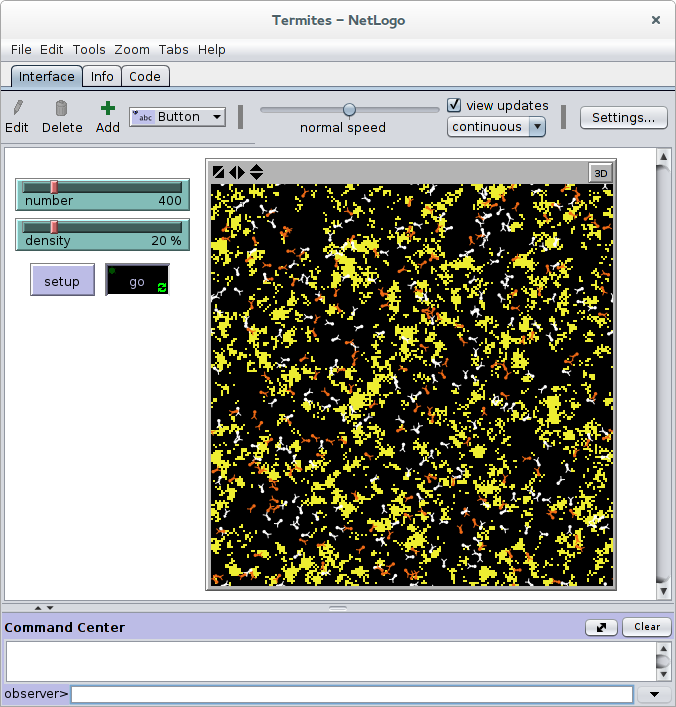
\includegraphics[scale=0.3]{doc/gestionProjet/netlogo-termites.png}
\caption{\label{netlogo-termites} Capture d'écran de NetLogo}
\end{figure}

Au début du projet, nous devions avoir une application graphique comparable à celle de NetLogo.

\begin{figure}[h]
\centering
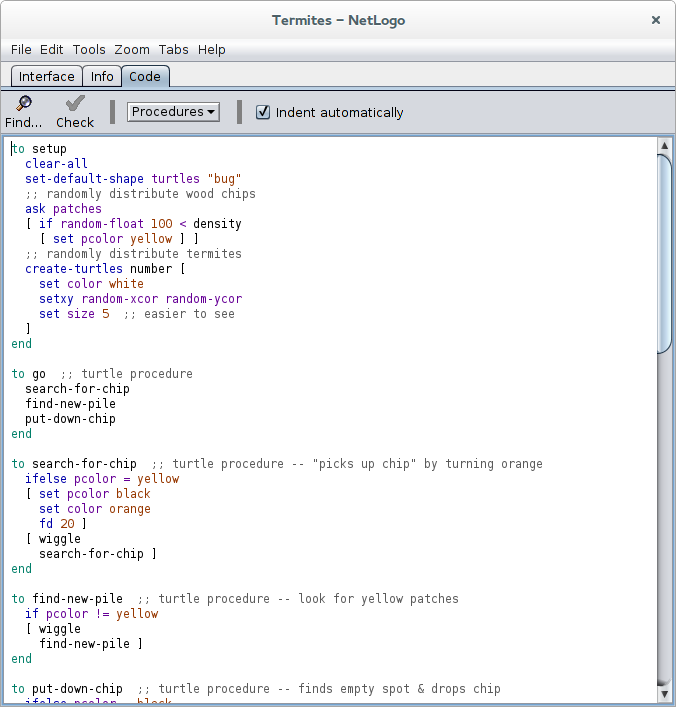
\includegraphics[scale=0.3]{doc/gestionProjet/netlogo-code.png}
\caption{\label{netlogo-code} L'éditeur de texte de NetLogo}
\end{figure}


Nous avions alors décidé de créer un langage où des tortues pourront bouger, communiquer entre elles et intéragir avec les zones. Une interface graphique pour observer une évolution de ces tortues était également prévue.

Au cours du projet, notre tuteur, Michel Meynard, nous a suggéré de rajouter l'exportation des données que nous manipulions~: le modèle (qui comprend l'ensemble des tortues, les zones et le monde). Nous avons donc rajouté cette possibilité à notre application, en l'ajoutant sur notre backlog.
Plus tard, nous avons aussi imaginé un programme complémentaire à notre application centré sur l'exportation de données~: un lancement à la console du programme, sans affichage graphique du déroulement de la simulation, mais avec des captures de cette simulation enregistré sous forme d'image et de JSON, pour les données.
Cela permet, lorsqu'on fait une simulation longue de ne pas utiliser les ressources graphiques de l'ordinateur. En outre, cela permet d'exécuter la simulation à pleine vitesse.
Un éditeur a été integré à l'interface graphique pour éditer le code et voir l'animation sans avoir deux programmes ouvert.
